\documentclass{article}
\usepackage{amsmath, amssymb, amsthm}
\usepackage[usenames,dvipsnames]{xcolor}
\usepackage{tikz-cd}
\usepackage{tikz, pgfplots}
\pgfplotsset{compat=1.18}
\usetikzlibrary{arrows.meta}
\usepgfplotslibrary{fillbetween}
\pgfdeclarelayer{ft}
\pgfdeclarelayer{bg}
\pgfsetlayers{bg, main, ft}

\begin{document}

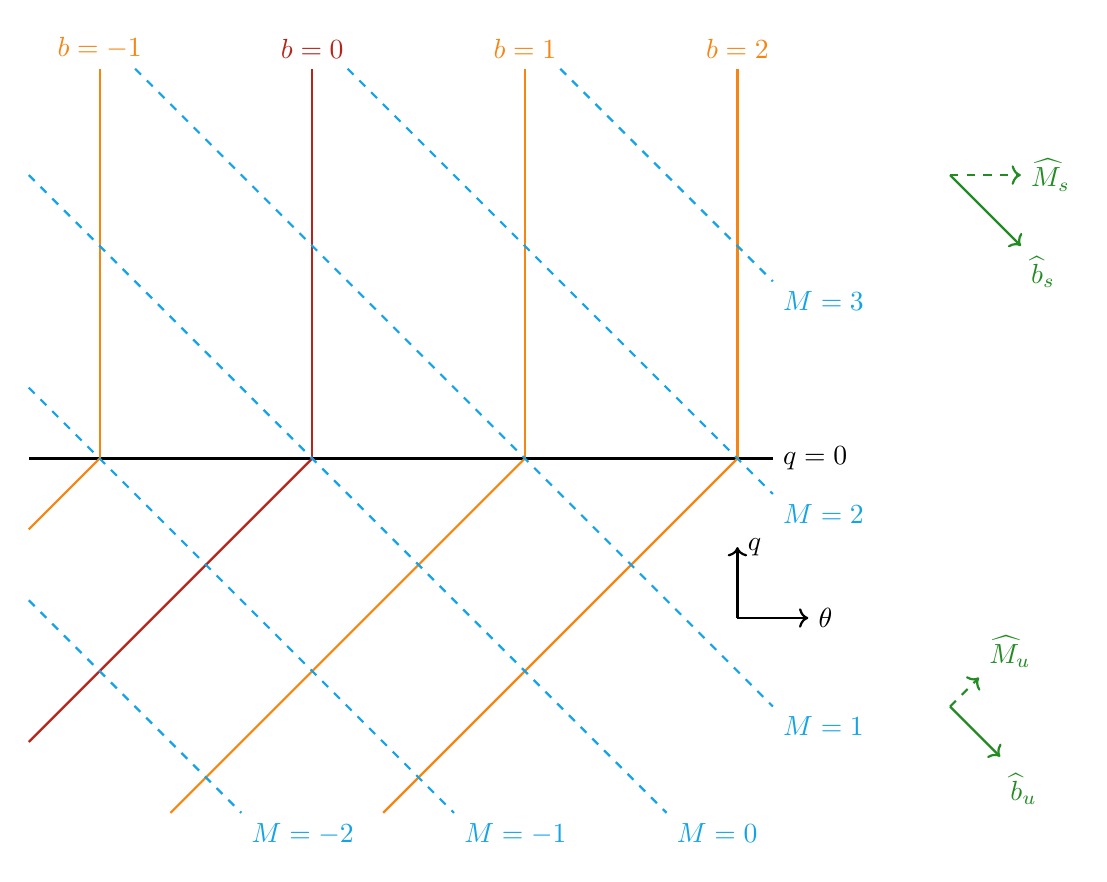
\begin{tikzpicture}[scale=0.9]
	% q = 0
	\draw[thick]		(-4, 0) --	( 6.5, 0);
	\node[thick, right] at			( 6.5, 0) {$q = 0$};

	% Coordinates theta and q
	\draw[thick, ->]	(6, -2.25) --	( 7, -2.25);
	\node[thick, right] at	       		( 7, -2.25) {$\theta$};
	\draw[thick, ->]	(6, -2.25) --	( 6, -1.25);
	\node[thick, right] at	     	  	( 6, -1.25) {$q$};

	% The sets of constant b

	% b = 0
	\draw[thick, BrickRed] (-4, -4) --	( 0, 0);
	\draw[thick, BrickRed] ( 0,  0) --	( 0, 5.5);
	\node[thick, above, BrickRed] at	( 0, 5.5) {$b=0$};

	% b = -1
	\draw[thick, BurntOrange] (-4  , -1  ) --	(-3, 0);
	\draw[thick, BurntOrange] (-3  ,  0  ) --	(-3, 5.5);
	\node[thick, above, BurntOrange] at		(-3, 5.5) {$b=-1$};

	% b = 1
	\draw[thick, BurntOrange] (-2, -5) --	( 3, 0);
	\draw[thick, BurntOrange] ( 3,  0) --	( 3, 5.5);
	\node[thick, above, BurntOrange] at	( 3, 5.5) {$b=1$};

	% b = 2
	\draw[thick, BurntOrange] ( 1, -5) --	( 6, 0);
	\draw[thick, BurntOrange] ( 6,  0) --	( 6, 5.5);
	\node[thick, above, BurntOrange] at	( 6, 5.5) {$b=2$};

	% The sets of constant M

	% M = 3
	\draw[dashed, thick, Cerulean] ( 3.5,  5.5) --		( 6.5,  2.5);
	\node[thick, Cerulean, below right] at		( 6.5,  2.5) {$M = 3$};

	% M = 2
	\draw[dashed, thick, Cerulean] ( 0.5,  5.5) -- 		( 6.5, -0.5);
	\node[thick, Cerulean, below right] at		( 6.5, -0.5) {$M = 2$};

	% M = 1
	\draw[dashed, thick, Cerulean] (-2.5,  5.5) -- 		( 6.5, -3.5);
	\node[thick, Cerulean, below right] at		( 6.5, -3.5) {$M = 1$};

	% M = 0
	\draw[dashed, thick, Cerulean] (-4  ,  4  ) --		( 5  , -5  );
	\node[thick, Cerulean, below right] at		( 5  , -5  ) {$M = 0$};

	% M = -1
	\draw[dashed, thick, Cerulean] (-4  ,  1  ) --		( 2  , -5  );
	\node[thick, Cerulean, below right] at		( 2  , -5  ) {$M = -1$};

	% M = -2
	\draw[dashed, thick, Cerulean] (-4  , -2  ) -- 		(-1  , -5  );
	\node[thick, Cerulean, below right] at		(-1  , -5  ) {$M = -2$};

	% Basis vectors (saturated region)
	\draw[dashed, thick, ForestGreen, ->]	( 9  , 4  ) --	(10  , 4  );
	\node[thick, ForestGreen, right] at		(10  , 4  ) {$\widehat{M}_s$};
	\draw[thick, ForestGreen, ->]	( 9  , 4  ) --	(10  , 3  );
	\node[thick, ForestGreen, below right] at	(10  , 3  ) {$\widehat{b}_s$};

	% Basis vectors (unsaturated region)
	\draw[dashed, thick, ForestGreen, ->]	( 9  ,-3.5) --	( 9.408,-3.092);
	\node[thick, ForestGreen, above right] at	( 9.408,-3.092) {$\widehat{M}_u$};
	\draw[thick, ForestGreen, ->]	( 9  ,-3.5) --	( 9.707,-4.207);
	\node[thick, ForestGreen, below right] at	( 9.707,-4.297) {$\widehat{b}_u$};

\end{tikzpicture}

\end{document}